\documentclass[tikz,border=2pt]{standalone}
\usepackage{amsmath}
\usepackage{pgfplots}
\pgfplotsset{compat=1.18}

\begin{document}
% A continuous function on a closed bounded interval [a,b] attains a largest and a smallest value
% (here the maximum at an interior point, the minimum at the endpoint b).
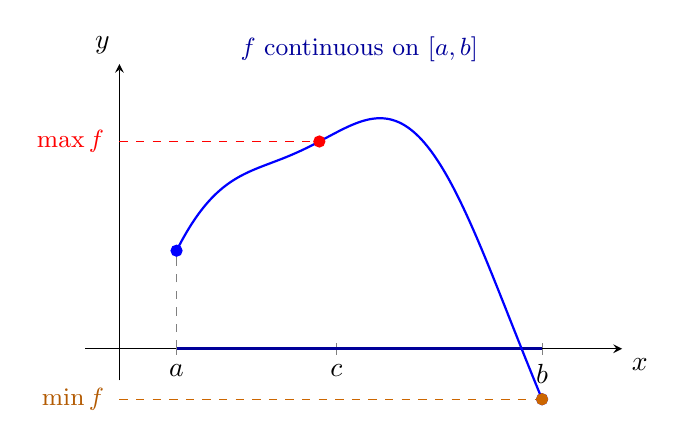
\begin{tikzpicture}
	\begin{axis}[
		axis lines=middle,
		xmin=-0.3, xmax=4.4,
		ymin=-0.4, ymax=3.6,
		xtick={0.5,1.9,3.7}, xticklabels={$a$,$c$,$b$},
		ytick=\empty,
		xlabel={$x$}, ylabel={$y$},
		xlabel style={below right}, ylabel style={above left},
		samples=150, smooth, clip=false,
		width=8.4cm, height=5.6cm
		]
		\draw[blue!60!black, very thick] (axis cs:0.5,0) -- (axis cs:3.7,0);
		\draw[dashed, gray] (axis cs:0.5,0) -- (axis cs:0.5,{2.9-1.96+0.3*sin(deg(1.5))});
		% f(x) = 3 - (x-1.9)^2 + 0.4 sin(3x): max near 1.9, min at b=3.7
		\addplot[thick, blue, domain=0.5:3.7] {2.9-(x-1.9)^2+0.3*sin(deg(3*x))};
		\addplot[only marks, mark=*, blue] coordinates {(0.5,{2.9-1.96+0.3*sin(deg(1.5))}) (3.7,{2.9-3.24+0.3*sin(deg(11.1))})};
		\addplot[only marks, mark=*, red] coordinates {(1.75,{2.9-0.0225+0.3*sin(deg(5.25))})};
		\addplot[only marks, mark=*, orange!80!black] coordinates {(3.7,{2.9-3.24+0.3*sin(deg(11.1))})};
		\draw[dashed, red] (axis cs:0,{2.9-0.0225+0.3*sin(deg(5.25))}) -- (axis cs:1.75,{2.9-0.0225+0.3*sin(deg(5.25))});
		\draw[dashed, orange!80!black] (axis cs:0,{2.9-3.24+0.3*sin(deg(11.1))}) -- (axis cs:3.7,{2.9-3.24+0.3*sin(deg(11.1))});
		\node[red, anchor=east, font=\small] at (axis cs:-0.05,{2.9-0.0225+0.3*sin(deg(5.25))}) {$\max f$};
		\node[orange!70!black, anchor=east, font=\small] at (axis cs:-0.05,{2.9-3.24+0.3*sin(deg(11.1))}) {$\min f$};
		\node[blue!60!black, anchor=south, font=\small] at (axis cs:2.1,3.5) {$f$ continuous on $[a,b]$};
	\end{axis}
\end{tikzpicture}
\end{document}
